\chapter{Úvod}
Práce byla vytvořena v rámci projektu informatika 2 ve spolupráci s občanským sdružením IuRe -- Iuridicum Remedium. Sdružení se zabývá ochranou soukromí a lidskými právy. Na svých stránkách\footnote{www.iure.org} zveřejňují mimo jiné \uv{výherce} ankety \texttt{Big brother awards} nebo webovou aplikaci mapa kamer\footnote{www.mapakamer.cz}, ve které zobrazují veřejná místa pokrytá kamerovými systémy. 
\begin{figure}[hb]
\begin{center}

\includegraphics[scale=0.3]{pics/iure_logo.png}
\caption{Logo občanského sdružení IuRe}
\end{center}
\end{figure}
\begin{figure}[hb]
\begin{center}
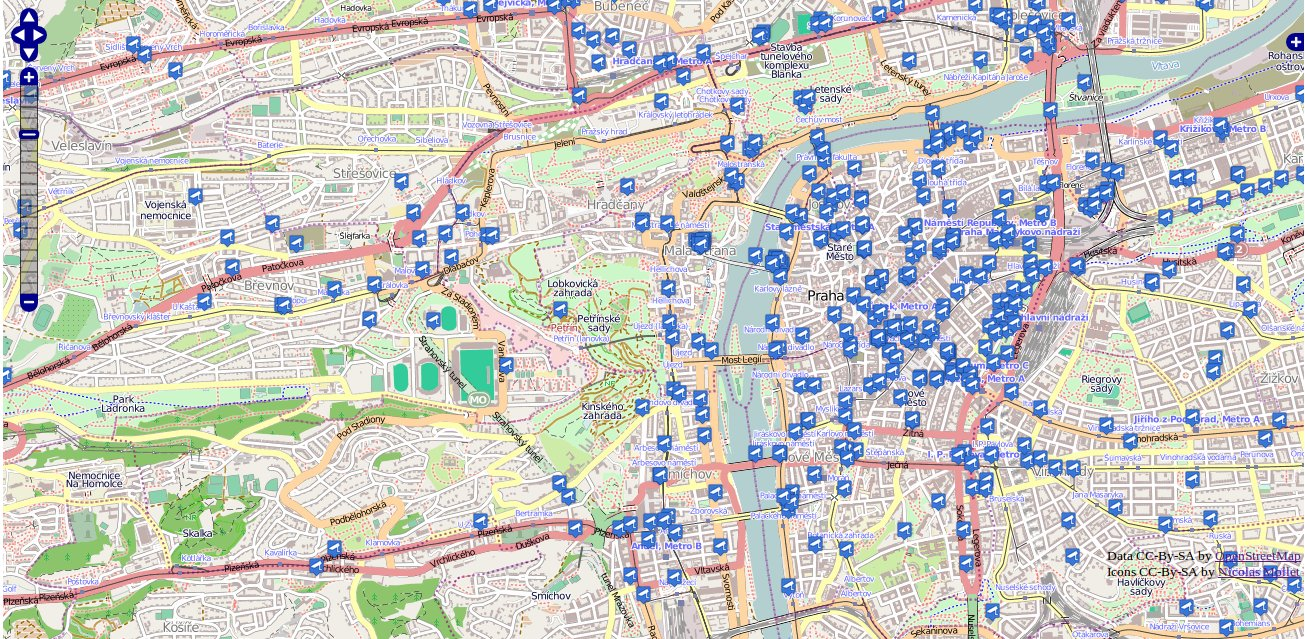
\includegraphics[scale=0.3]{pics/mapakamer.jpg}
\caption{Webová aplikace Mapa kamer}
\end{center}
\end{figure}
\paragraph{}
Sdružení se již v minulosti pokoušelo o tvorbu mobilní aplikace pro zaznámenávání a zobrazování kamer, ale potýkalo se s nedostatkem pracovních kapacit, proto naši bezplatnou nabídku ke spolupráci rádi přijali. Základ aplikace byl již připraven, ale nespl\v{n}oval ani jejich ani naše očekávání. Aplikace byla založena na \texttt{Google Maps} a neměla v pozadí ani databázi, ani server. I o to jsme se tedy museli postarat. 
\paragraph{}
Aplikace je zacílena na mobilní operační systém \texttt{Android}. Jazykem běžně používaným pro tvorbu aplikací pro \texttt{Android} je \texttt{Java}. Použili jsme vývojové prostředí \texttt{Eclipse}, do kterého je však pro tvorbu mobilních aplikací potřeba doinstalovat \texttt{Android Developer Tools}.
\begin{figure}[hb]
\begin{center}

\includegraphics[scale=0.1]{pics/android.jpg}
\end{center}
\end{figure} 
\paragraph{}
Jako podkladová mapa byly použity rastry z opensourcového projektu \texttt{OpenStreetMap}\footnote{www.openstreetmap.org}. Pro uchovávání informací o kamerách byla použita databáze \texttt{PostgreSQL} a dále byla, opět v jazyce \texttt{Java}, napsána webová aplikace umož\v{n}ující komunikaci mezi mobilním zařízením a databází.